\documentclass[11pt]{article}

\usepackage[utf8]{inputenc}
\usepackage[T1]{fontenc}

\usepackage[a4paper, left=2cm, right=2cm, top=3.5cm, bottom=3.5cm]{geometry}
\usepackage[french]{babel}

% Paragraph spacing
\setlength{\parskip}{1em}

% Fancy headers
\usepackage{fancyhdr}

% Captions for subfigures
\usepackage{subcaption}

% Code highlighting
\usepackage{minted}

% Footnote inside a caption
\usepackage{fnpos}
\usepackage{ftnxtra}

% Maths
\usepackage{amsmath}
\usepackage{amssymb}

% Todo notes
\usepackage{todonotes}

% Table of contents for bibliography
\usepackage[nottoc]{tocbibind}

% Inline monospace font
\def\code#1{\texttt{#1}}

% Figures
\usepackage{graphicx}

% Draw figures
\usepackage{tikz}

% Tikz node rotation
\usetikzlibrary{positioning}

% Turing machine
\usetikzlibrary{chains,fit,shapes}

% Usage: \rotnode[options]{rotation}{text}
\newcommand\rotnode[3][]{%
    \node [#1, opacity=0.0] (tmp) {#3};
    \node [draw, rotate around={#2:(tmp.center)}] at (tmp) {#3};
}

% Clickable links
\usepackage{hyperref}

% Table of contents depth
\setcounter{tocdepth}{2}

% Inline code
\usepackage{listings}
\usepackage{color}

\title{Systèmes d'exploitation : moniteurs}

\author{William SCHMITT}
\date{2018-2019}

\begin{document}
\maketitle

\section{Introduction}
Les \textbf{moniteurs} permettent de faire de la synchronisation de \textbf{threads} : un même programme, dont la mémoire est partagée.

On considère un ensemble de fonctions en exclusion mutuelle. On peut faire attendre un thread, tant que l'état d'un système n'est pas propice à son exécution. Cette contradiction est gérée par des variables de condition, dont le rôle est d'organiser une file d'attente de threads.

\section{Exercices}
Il s'agit de comprendre le fonctionnement de ces cas, qui sont déjà implantés dans les bibliothèques standard.

\subsection{Barrière à N}
Des threads attendent à une barrière, lorsqu'il y en a N qui sont à la barrière, tous les N continuent.

On a besoin de : 
\begin{itemize}
    \item Mutex pour l'exclusion mutuelle
    \item Compteur pour connaître le thread
    \item Variable de condition pour savoir quand attendre/partir
\end{itemize}

\begin{figure}[ht]
    \centering
    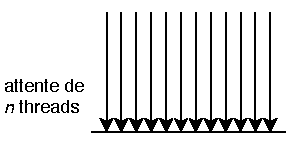
\includegraphics{img/cours5/barriere.pdf}
    \caption{Barrière à N}
\end{figure}

\begin{minted}[frame=single]{C}
const N = 42;
int compteur = 0
mtx_t m;
cnd_t c;

void barriereN() {
    mtx_lock(&m);
    compteur++;
    while (compteur < N) { // On aurait également pu utiliser if ici
        // le compteur++ peut également être là
        cnd_wait(&c, &m);
    }
    cnd_signal(&c);
    mtx_unlock(&m);
}
\end{minted}

\paragraph{Remarque :} \mintinline{c}{cnd_signal()} réveille un thread à la fois. On observe donc ici un réveil en cascade (le dernier réveille le premier, qui réveille le second etc.).

\paragraph{Remarque 2 : } le $N+1$ème thread passe directement, la barrière est donc à usage unique.

\subsection{Allocateur}
On ne s'occupe pas de la façon d'utiliser les fonctions, il y a cependant des détails à connaître :
\begin{itemize}
    \item Les ressources ne sont pas infinies : il est possible de devoir attendre dans \mintinline{c}{allocation}
    \item Il n'y a pas d'attente pour \mintinline{c}{liberation}
\end{itemize}

On se contente de réveiller tous les threads en attente dans \mintinline{c}{allocation}, et on laisse les threads vérifier si assez de ressources sont disponibles.

Une autre fonction existe : \mintinline{c}{void cnd_broadcast(cnd_t * c)}, qui débloque toute une file.

\begin{minted}[frame=single]{C}
    int resource = N;
    mtx_t m;
    cnd_t c;

    void allocation(int n) {
        mtx_lock(&m);
        while (resource < n) {
            cnd_wait(&c, &m);
        }
        resource -= n;
        mtx_unlock(&m);
    }

    void liberation(int n) {
        mtx_lock(&m);
        resource += n;
        cnd_broadcast(&c);
        mtx_unlock(&m);
    }
\end{minted}

Ce code est susceptible de créer des famines : pour un ensemble de threads demandant 1, sauf un qui demande 2, ce dernier pourrait ne jamais partir.

On peut essayer de faire du réveil en cascade. Dans la sémantique de Hoare le signal est bloquant, mais en réalité signal n'est jamais implanté de façon bloquante, ce code est donc \textbf{FAUX}. Dans le cas où l'on a 2 threads qui demandent trop de ressources, ils peuvent se renvoyer la balle constamment, se réveillant l'un l'autre.
\begin{minted}[frame=single]{C}
    // CODE FAUX - ILLUSTRATION
    int resource = N;
    mtx_t m;
    cnd_t c;

    void allocation(int n) {
        mtx_lock(&m);
        while (resource < n) {
            cnd_wait(&c, &m);
            cnd_signal(&c); // réveille le suivant
        }
        resource -= n;
        mtx_unlock(&m);
    }

    void liberation(int n) {
        mtx_lock(&m);
        resource += n;
        cnd_signal(&c); // réveille le premier
        mtx_unlock(&m);
    }
\end{minted}

\subsection{Producteur-consommateur}

\begin{figure}[ht]
    \centering
    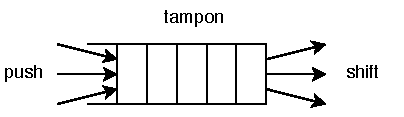
\includegraphics{img/cours5/tampon.pdf}
    \caption{Tampon}
\end{figure}
Un producteur est un tampon (de taille bornée). On peut l'implanter de diverses manières, mais on utilise ici un tampon circulaire, un tableau de taille N utilisé avec deux indices : un indice de lecture et un indice d'écriture. On ne peut pas différencier le cas "tableau vide" du cas "les deux indices ont été incrémentés n fois". On se munit donc d'une autre variable : le nombre de messages déposés dans le tableau.

On sépare la file en deux, de façon à savoir qui on réveille.

\begin{minted}[frame=single]{c}
int iecr = 0;
int ilect = 0;
int nb = 0;
mtx_t m;
cnd_t fp; // File pour les producteurs
cnd_t fconso; // File pour les consommateurs

void push(Msg msg) {
    mtx_lock(&m);
    mtx_unlock(&m);
}

Msg shift() {
    mtx_lock(&m);
    mtx_unlock(&m);
}
\end{minted}

\end{document}